\documentclass[11pt]{article}
%\usepackage[version=3]{mhchem} % Package for chemical equation typesetting
%\usepackage{siunitx} % Provides the \SI{}{} and \si{} command for typesetting SI units
%\usepackage{graphicx} % Required for the inclusion of images
%\usepackage{natbib} % Required to change bibliography style to APA
\usepackage{amsmath} % Required for some math elements 
\usepackage[margin=1in]{geometry}
\usepackage{microtype}
\usepackage[english]{babel}
\usepackage[utf8]{inputenx}
\usepackage{float}
\usepackage{graphics}
\usepackage{graphicx}
\usepackage{subfigure}
\usepackage{amsmath}
\usepackage{textcomp}
\usepackage{makeidx}
\usepackage{hyperref}
\usepackage{braket}
%\usepackage[latin1]{inputenc}
\usepackage{amsthm}
\usepackage{amsfonts}
\usepackage{amssymb}
\usepackage{graphicx}
\usepackage{fullpage}
\usepackage{hyphenat}
\usepackage{float}
\usepackage{longtable}
\usepackage{picture}
\usepackage{multicol}
\usepackage{fancyhdr}
\usepackage{wrapfig}
\usepackage{geometry}
\usepackage{listings}
\usepackage{color}
\definecolor{dkgreen}{rgb}{0,0.6,0}
\definecolor{gray}{rgb}{0.5,0.5,0.5}
\definecolor{mauve}{rgb}{0.58,0,0.82}

\lstset{frame=tb,
	language=C++,
	aboveskip=3mm,
	belowskip=3mm,
	showstringspaces=false,
	columns=flexible,
	basicstyle={\small\ttfamily},
	numbers=none,
	numberstyle=\tiny\color{gray},
	keywordstyle=\color{blue},
	commentstyle=\color{dkgreen},
	stringstyle=\color{mauve},
	breaklines=true,
	breakatwhitespace=true,
	tabsize=3
}

\theoremstyle{theorem}
\newtheorem{theorem}{Theorem}
\newtheorem{proposition}{Proposition}

\theoremstyle{definition}
\newtheorem{definition}{Definition}



%\usepackage{tikz}
%\usetikzlibrary{graphs}
%\usepackage{pgfplots}
%\pgfplotsset{compat=newest}

\setlength\parindent{0pt} % Removes all indentation from paragraphs

\renewcommand{\figurename}{Grafico}
\renewcommand{\tablename}{Tabella}
\newcommand{\at}[2][]{#1\Big|_{#2}}
\renewcommand{\labelenumi}{\alph{enumi}.} % Make numbering in the enumerate environment by letter rather than number (e.g. section 6)

%\usepackage{times} % Uncomment to use the Times New Roman font

%----------------------------------------------------------------------------------------
%	DOCUMENT INFORMATION
%----------------------------------------------------------------------------------------

\title{C1 - Assignment 3 Report: Scalar initial value problems.} % Title

\author{Student Number: 1894945} % Author name

\date{\today} % Date for the report

\begin{document}

\maketitle % Insert the title, author and date

\begin{center}
C1 - Assignment 3 Report \hfill
Student Number: 1894945
\vspace{3pt} \hrule \vspace{3pt} \hrule
\end{center}

%\clearpage
\tableofcontents

\clearpage
% If you wish to include an abstract, uncomment the lines below
%\begin{abstract}


%\end{abstract}
%\clearpage 

\section{Introduction}
In this assignment the approximation of solutions to the Cauchy problem
for scalar ordinary differential equations (ODEs) will be considered.

\begin{definition}
	\label{def:Cauchy-prob}
	Let $I\subset\mathbb{R}$ be an interval, $t_0\in I$, $f(t,y):I\times\mathbb{R}\rightarrow\mathbb{R}$. The initial value problem (IVP) for a first order ODE is to find a function $y\in C^1(I)$, such that:
	\begin{align}
		\label{eqn:Cauchy-prob}
		\begin{cases}
		y'(t)=f(t,y(t)),\hspace{4mm}\forall t\in\mathbb{R}\\
		y(t_0)=y_0
		\end{cases}
	\end{align} 
	for the initial condition $y_0\in\mathbb{R}$. If $f$ does not explicitly depend on
	$t$ (but only through $y(t)$) the IVP is called autonomous.
\end{definition}

The following theorem provides sufficient conditions for the existence and uniqueness of solutions to Problem (\ref{def:Cauchy-prob}).\\

\begin{theorem}
	\label{thm:Picard}
	If $f(t,y(t))$ is continuous in t, the IVP (\ref{def:Cauchy-prob}) admits a unique global solution if there exists a constant $L>0$ independent of t such that
	\begin{align}
		\label{eqn:Lipschitz}
		|f(t,y_1)-f(t,y_2)|\le L|y_1-y_2|\hspace{5mm}\forall t\in I,\hspace{3mm} y_1,y_2\in\mathbb{R}
	\end{align}
\end{theorem}

Stability can be formulated in the following way.

\begin{definition}
	\label{def:stability}
	Consider the following perturbed IVP:
	\begin{align}
	\label{eqn:pert-prob}
	\begin{cases}
	z'(t)=f(t,z(t))+\delta(t),\hspace{4mm}\forall t\in\mathbb{R}\\
	z(t_0)=y_0+\delta_0
	\end{cases}
	\end{align}
	where both the initial condition and the function $f$ are perturbed. IVP (\ref{def:Cauchy-prob}) is stable, if for any perturbation $(\delta_0, \delta(t))$ staisfying $|\delta_0|<\varepsilon$, $|\delta(t)|<\varepsilon\hspace{3mm}\forall t\in I$, $\varepsilon$ bein small enough to guarantee a unique solution for the problem still exists, $\exists$ $C>0$ such that 
	
	$$|y(t)-z(t)|<C\varepsilon\hspace{5mm}\forall t\in I$$ 
\end{definition}

It is worth making note that the Lipschitz property of $f$ implies stability of Problem (\ref{def:Cauchy-prob}), as it can be shown by means of the Gronwall lemma.\\

Since a discrete version of the Gronwall lemma will be needed in the following to prove
stability of discrete schemes, it is convenient to introduce such a variation immediately.

\begin{theorem}
	\label{thm:Gronwall-discrete}
	Let $\alpha_n$ and $\beta_n$ be two non-negative sequences, $g_0\ge 0$ and $u_n$ a sequence such that:
	\begin{align}
	\begin{cases}
	u_0\le g_0\\
	u_n\le g_0 + \sum_{s=0}^{n-1}\alpha_s + \sum_{s=0}^{n-1}\beta_su_s, \hspace{4mm}n\ge 1
	\end{cases}
	\end{align}
	Then:
	\begin{align*}
		u_n\le\left(g_0 + \sum_{s=0}^{n-1}\alpha_s\right)exp{\left(\sum_{s=0}^{n-1}\beta_s\right)}	\end{align*}
\end{theorem}

\subsection{One-step methods}
In the following, the integration interval $I=[t_0, t_0+T]$ will be discretised with $N$ evenly spaced intervals $I_n=[t_n, t_{n+1}]$ , where $t_n=t_0+nh$. The quantity $h=|I_n|$ is called the discretisation stepsize. It is worth making notice that it has not been required that $h=\frac{T}{N}$, i.e. it is possible that $t_N\ge t_0 + T$.
At each node $t_i$, let $u_i$ be the approximation of the solution $y(t_i)=y_i$. Additionally, denote $f(t_i,u_i)=f_i$.\\

\begin{definition}
	\label{def:One-step-method}
	A numerical method approximating IVP (\ref{def:Cauchy-prob}) is called one-step method, if $\forall n\ge 0$, $u_{n+1}$ depends only on $u_n$. The method is called multi-step method otherwise.
\end{definition}

In the present assignment the following one-step methods are used.\\

\begin{definition}[Forward Euler Method]
	\label{def:FE}
	\begin{align}
	\begin{cases}
	\label{eqn:FE}
	u_0=y_0\\
	u_{n+1}=u_n+hf_n
	\end{cases}
	\end{align}
\end{definition}

\begin{definition}[Backward Euler Method]
	\label{def:BE}
	\begin{align}
	\begin{cases}
	\label{eqn:BE}
	u_0=y_0\\
	u_{n+1}=u_n+hf_{n+1}
	\end{cases}
	\end{align}
\end{definition}

\begin{definition}[Heun Method]
	\label{def:Heun}
	\begin{align}
	\begin{cases}
	\label{eqn:Heun}
	u_0=y_0\\
	u_{n+1}=u_n+\frac{h}{2}(f_n+f(t_{n+1}, u_n+hf_n))
	\end{cases}
	\end{align}
\end{definition}

Of the above methods, the forward Euler method and the Heun method are explicit,
while the backward Euler method is implicit.

\begin{definition}
	\label{def:implicit-explicit}
	A method is called explicit, if $u_{n+1}$ can be computed directly in terms of previous values $u_k$, $k<n$. It is called implicit, if $u_{n+1}$ implicitly depends on itself through f.
\end{definition}

\subsection{Zero Stability}
Explicit one-step methods can be always written as:

\begin{align}
	\label{eqn:one-step-method}
	u_{n+1}=u_n+h\Phi(t_n,u_n,f_n;h)\hspace{5mm}0\le n\le N-1,\hspace{3mm}u_0=y_0
\end{align}

If we additionally call $y_n=y(t_n)$, the restriction of the solution of the IVP to our
temporal discretisation becomes:

$$y_{n+1}=y_n+h\Phi(t_n,u_n,f(t_n, y_n);h)+\varepsilon_{n+1}\hspace{5mm}0\le n\le N-1,\hspace{3mm}u_0=y_0$$

where $\varepsilon_{n+1}$ is the residual at the node $t_{n+1}$. In general, since every numerical method only approximates the continuous IVP, one cannot expect it to transform $y_n$ into $y_{n+1}$ precisely, and thus the residual will be non-zero.\\

\begin{definition}
	\label{def:truncation-error}
	The quantity:
	\begin{equation}
		\label{eqn:local-truncation-error}
		\tau_n(h)=\frac{\varepsilon_n}{h}
	\end{equation}
	is called the local truncation error (LTE) at the node $t_n$. Consequently, the global truncation error is defined as:
	\begin{equation}
	\label{eqn:global-truncation-error}
	\tau(h)=\max\limits_{0\le n\le N-1}|\tau_{n+1}(h)|
	\end{equation}
\end{definition}

The following definition is also of extreme importance for numerical IVPs.

\begin{definition}
	\label{def:consistency}
	A method is said to be consistent if:
	$$\tau(h)\rightarrow 0\hspace{3mm}\text{for}\hspace{3mm}h\rightarrow 0$$
	Moreover, a scheme has a consistency order $p$ if:
	$$\tau(h)=\mathcal{O}(h^p)\hspace{3mm}\text{for}\hspace{3mm}h\rightarrow 0$$
\end{definition}

One can now introduce the following.

\begin{definition}
	\label{def:zero-stability-one-step}
	A one-step method is zero-stable if $\exists h>0$, $\exists C>0$ such that $\forall h\in (0, h_0]$, $\forall\varepsilon>0$ sufficiently small:
	
	$$|\delta_n|\le\varepsilon\implies |z_n-u_n|\le C\varepsilon$$
	
	where $z_n$ and $u_n$ are the solutions of:
	
	\begin{align*}
	\begin{cases}
	z_{n+1}=z_n+h\left(\Phi(t_n, z_n, f(t_n, z_n);h)+\delta_{n+1}\right)\\
	z_0=y_0+\delta_0
	\end{cases}
	\end{align*}
	
	and 
	
	\begin{align*}
	\begin{cases}
	u_{n+1}=u_n+h\left(\Phi(t_n, z_n, f(t_n, u_n);h)\right)\\
	u_0=y_0
	\end{cases}
	\end{align*}
	
	for $0\le n\le N$.
	This property ensures that the numerical method is robust against small changes in
	the data and thus corresponds to the notion of stability defined more generally earlier. Again, one requests stability of a numerical method because it implies weak sensitivity with respect to unavoidable errors because of the computer’s finite arithmetic accuracy.
\end{definition}

\begin{theorem}
	\label{thm:zero-stability}
	Consider a one-step method for an IVP. Assuming that for the increment function $\Phi$, $\exists h_0>0$, $\Lambda>0$ such that $\forall h\in(0, h_0]$
	
	
	$$|\Phi(t_n, u_n, f(t_n, u_n);h)-\Phi(t_n, z_n,f(t_n, z_n);h)|\le\Lambda|u_n-z_n|$$
	
	for $0\le n\le N$, i.e. that $\Phi$ is Lipschitz continuous with respect to its second argument. Then the one-step method is zero-stable.\\
\end{theorem}

\begin{proof}
	See Ref.(\cite{lec-notes}).
\end{proof}


\subsection{Convergence analysis}
\begin{definition}
	\label{def:convergence}
	A method is said to be convergent if 
	
	$$|y_n-u_n|\rightarrow 0\hspace{2mm}\text{as}\hspace{2mm}h\rightarrow 0\hspace{3mm}\forall n\in\lbrace 1,\cdots, n\rbrace$$
	
	and is said to be convergent of order $p$ if 
	
	
	$$|y_n-u_n|\rightarrow 0\hspace{2mm}\text{as}\hspace{2mm}h\rightarrow \mathcal{O}(h^p)\hspace{3mm}\forall n\in\lbrace 1,\cdots, n\rbrace$$
\end{definition}

\begin{theorem}[Convergence for one-step methods]
	\label{thm:convergence-one-step}
	Under the same assumptions as in Thm.\ref{thm:zero-stability} and the additional assumption that 
	
	$$|y_0-u_0|\leftarrow h=0\hspace{4mm}h\rightarrow 0$$
    then the corresponding one-step method is convergent. More precisely, one has:
    
    \begin{align}
    	\label{eqn:convergence-one-step}
    	|y_n-u_n|\le\left(|y_0-u_0)|+nh\tau (h)\right)e^{nh\Lambda},\hspace{5mm}1\le n\le N
    \end{align}
    
    Moreover, if the one-step method has consistency order p and $|y_0-u_0|=\mathcal{O}(h^p)$, then the method is also convergent with order p.\\
\end{theorem}

\begin{proof}
	See Ref.(\cite{lec-notes}).
\end{proof}

\subsection{Absolute stability}
In opposition to the property of zero-stability, the concept of absolute stability can be introduced. Loosely, a numerical method is absolutely stable if, for a fixed stepsize
$h$, $u_n$ remains bounded as we let $t_n\rightarrow\infty$. In short, for absolute stability, one looks at the asymptotic behaviour of $u_n$ for long times, whereas zero-stability deals with a fixed integration interval, but considers $h\rightarrow 0$.\\
In order to define absolute stability, the following, very particular IVP is introduced: 

\begin{align}
\label{eqn:test-problem}
\begin{cases}
y'(t)=\lambda y(t),\hspace{5mm}t>0\\
y(0)=1
\end{cases}
\end{align}

where $\lambda\in\mathbb{C}$. Eqn.\eqref{eqn:test-problem} defines the \emph{test problem}.\\
The solution to the test problem obviously is $y(t)=e^{\lambda t}$. In particular, we have $|y(t)|\rightarrow 0$ as $t\rightarrow \infty$ only if $Re(\lambda)<0$. For a general $\lambda\in\mathbb{C}$, the test problem captures the combined effect of decay or growth with simulations oscillation and it turns out to be informative to analyse how well our numerical solutions are able to approximate the correct solution depending on the choice of $\lambda$ in the complex plane.\\

\begin{definition}[Absolute Stability]
	\label{def:abs-stability}
	A numerical method for approximating the test problem \eqref{eqn:test-problem} is called absolutely stable for a given $\lambda\in\mathbb{C}$ and stepsize $h>0$, if:
	
	$$|u_n|\rightarrow 0,\hspace{3mm}\text{for}\hspace{3mm} t_n\rightarrow\infty$$	 
\end{definition}

The numerical approximation $u_n$ depends on the stepsize $h$ and on the test problem parameter $\lambda$. A method will be absolutely stable only for certain values of $h$ and on the test problem parameter $\lambda$. A method will be absolutely stable only for certain values of $h$ and $\lambda$. 

\begin{definition}
	\label{def:region-abs-stab}
	The region of absolute stability of a method is the complex plane region $\mathcal{A}\subset\mathbb{C}$ such that:
	$$ \mathcal{A}=\lbrace z=h\lambda\in\mathbb{C}: \text{the method is absolutely stable} \rbrace$$
\end{definition}

\begin{definition}[A-stability]
	\label{def:A-stability}
	A method is said to be A-stable if
	$$\mathcal{A}\cap\mathbb{C}^{-}=\mathbb{C}^{-}$$
	where $\mathbb{C}^{-}=\lbrace z\in\mathbb{C}\hspace{1mm}|\hspace{1mm}Re(z)<0\rbrace$ and $\mathcal{A}$ is the region of absolute stability of the method.\\ 
\end{definition}
 
In other words, a method is A-stable if $|u_n|\rightarrow 0$ as $t_n\rightarrow\infty$ for all $\lambda$ with negative real part.\\

\subsection{Runge-Kutta methods}
In the present assignment, Runge-Kutta (RK) methods are employed.\\
\begin{definition}[Runge-Kutta methods]
	\label{def:RK}
	RK methods are one-step methods of the form:
	$$u_{n+1}=u_n + hF(t_n, u_n, f, h)$$
	where the increment function $F$ is defined as
	$$F(t_n, u_n, f, h)=\sum_{i=1}^{s}b_iK_i$$
	for
	\begin{align}
		\label{eqn:Ki}
		K_i=f\left(t_n + hc_i, u_n + h\sum_{j=1}^{s}a_{ij}K_j\right)\hspace{4mm}i\in\lbrace1,\dots s\rbrace
	\end{align}
	The integer $s$ stands for the number of stages of the method.\\
\end{definition}

It is worth to make notice of both the fact that the coefficients $A=(a_{ij})\in\mathbb{R}^{s\times s}$, $b\in\mathbb{R}^s$ and $c\in\mathbb{R}^s$ completely determine the RK method and of the fact that Eqn.\eqref{eqn:Ki} is an implicit equation for $K_i$.\\
\begin{definition}
	\label{def:Butcher-tableau}
	An RK method is completely described by the Butcher tableau:\\
		\begin{align*}
			\begin{tabular}{c|c}
			$\mathbf{c}$ & A  \\
			\hline
			& $\mathbf{b}^T$ \\
			\end{tabular}
			=
			\begin{tabular}{c|c}
			$c_1$ & $a_{11}\cdots a_{1s}$  \\
			$\vdots$ & \vdots\hspace{5mm} \vdots \\
			$c_s$ & $a_{s1}\cdots a_{ss}$ \\
			\hline
			& $b_1\cdots b_s$ \\
			\end{tabular}
		\end{align*}
	
\end{definition}
An RK method is explicit, if each $K_i$ can be explicitly computed in terms of the coefficients $K_1,\dots ,K_{i-1}$ that have already been determined.\\
As usual, consistency is defined by looking at the local truncation error, which in turn
is obtained by computing the discrepancy when inserting the solution $y$ into the method.\\

The following theorems, whose proof can be found in Ref.\cite{lec-notes}, are fundamental to characterise the properties of an RK method.\\

\begin{theorem}
	\label{thm:consistency-RK}
	An RK method is consistent if $\sum_{i=1}^{s}b_i=1$.
\end{theorem}

\begin{theorem}[Maximal order of an RK method]
	\label{thm:order-RK}
	The following upper-bounds can be found for the order of consistency of RK methods:
	\begin{itemize}
		\item The order of consistency of an explicit s-stage-RK method is at most s;
		\item The order of consistency of an s-stage implicit method is at most 2s.
	\end{itemize}
\end{theorem}

\begin{theorem}[Order conditions for RK methods]
	\label{thm:order-cond-RK}
	Consider an s-stage-RK method with Butcher tableau 
	\begin{tabular}{c|c}
		$\mathbf{c}$ & A  \\
		\hline
		& $\mathbf{b}^T$ \\
	\end{tabular}
	. The method is order p iff $\forall q\in\lbrace 1,\cdots, p\rbrace$ the following conditions hold true:
	\begin{itemize}
		\item Order 1: $\sum_{i=1}^{s}b_i=1$;
		\item Order 2: $\sum_{i=1}^{s}b_ic_i=\frac{1}{2}$;
		\item Order 3: $\sum_{i=1}^{s}b_ic_i^2=\frac{1}{3}$ and $\sum_{i=1}^{s}\sum_{j=1}^{s}b_ia_{ij}c_j=\frac{1}{6}$;
	\end{itemize}
	For greater orders, more conditions are needed.\\
\end{theorem}

Being that RK methods are one-step methods, their zero-stability comes from Thm.\ref{thm:zero-stability}, whereas their consistency is guaranteed by construction,
e.g. by adhering to the conditions of Thm.\ref{thm:order-cond-RK}., their convergence can be studied through the fundamental theorem.\\
\subsubsection{Absolute stability for RK methods}
The absolute stability of an RK method can be investigated by its stability function
$R:\mathbb{C}\rightarrow\mathbb{C}$:
\begin{align}
	\label{eqn:R}
	R(z)= 1+z\mathbf{b}^T(I-zA)^{-1}\mathbf{e}
\end{align}
where $A$ and $\mathbf{b}$ are given by the method's Butcher tableau, $\mathbf{e}=(1,\cdots, 1)^T\in\mathbb{R}^s$ and $I\in\mathbb{R}^{s\times s}$ is the identity matrix.

\begin{theorem}
	\label{thhm:sol-evol-RK}
	If an RK method is applied to the test problem \eqref{eqn:test-problem}, then the numerical solution evolves according to:
	$$u_{n+1}=R(h\lambda)u_n,\hspace{5mm}n\in\lbrace1,\cdots,N\rbrace$$
	where $R$ is the method's stability function.\\
\end{theorem}

With this knowledge, the region of absolute stability is easily determined: an RK
method is absolutely stable for

$$ z=h\lambda\in\mathbb{C} $$

iff

$$||R(z)||<1$$

Hence, the region of absolute stability of an RK method is:

$$A=\lbrace z\in\mathbb{C}:||R(z)||<1\rbrace$$


\section{The program}
\subsection{Implementation}
The program is built on the classes and struct contained in the files \emph{schemes.hh} and \emph{models.hh}, which contain the different RK method employed to find a solution and the different benchmark problem to test on, respectively.\\
\subsubsection{schemes.hh file}
\label{subsubsec:schemes}
The class DIRK is made of 4 \emph{protected} variables: the matrix $A$, the vector $b$, the vector $c$ and the integer $s$, which fully characterise the Butcher tableau of any RK method. This is done through the following instructions, which can be found in the schemes.hh file:

\begin{lstlisting}
protected:

	int stages_;

	std::vector<double> a_,b_,c_;
\end{lstlisting}

It may be worth pointing out that, even though \emph{a$\_$} represents a matrix, it is implemented as a vector in the program.\\
The classes $FE$, $BE$, $IM$, $Heun3$ and $DIRK2$ are implemented as derived classes of $DIRK$, being that all of them represent particular instances of such a class.\\

The function \emph{evolve}, which returns the evolved approximated solution $u_{n+1}$, $u_n$ being the present approximation, can be found in the file as well. For flexibility reasons, the function is built as a \emph{template}: in this way, both methods can be accessed by the function. The prototype of the routine, is displayed in the following:

\begin{lstlisting}
double evolve(const double &y,double t,double h,const Model &model,unsigned &count) const //one step forward
\end{lstlisting}

Here $y$ represents the approximated solution at the time $t$, with $h$ the chosen discretisation stepsize.\\
In case an implicit RK method is chosen, Eqn.\ref{eqn:Ki} becomes an implicit equations for $K_i$ and has to be solved by means of numerical methods. Here, Newton's method is has been employed.\\

\begin{lstlisting}
if( a(i,i)!=0 ) //implementing newton method
{
	unsigned iter = 0;
	double error = ( -k[i] + model.f(t + c_[i]*h, tmp_sum + h*a(i,i)*k[i]) );
	count ++;
	double den; //den stays for the denumerator of the fraction which updates k[i] in Newton's method
	while(iter < 1e6 && std::abs(error) > 1e-6 ) //1e6 is maximum number of iterations and 1e-6 is the given tol
	{
		den = -1 + model.df( t + c_[i]*h, tmp_sum + k[i] )*h*a(i,i);
		count++;
		k[i] -= error/den;
		error = -k[i] + model.f(t + c_[i]*h, tmp_sum + h*a(i,i)*k[i]) ;
		count++;
	iter ++;
	}
\end{lstlisting}

As it can be seen from the listed code above, the program checks if the chosen method happens to be implicit: if the entry $a_{ii}\neq 0$, then Newton's method is implemented. The error at every iteration, which is equal to $f\left(t+hc_i, u_n+h\sum_{j=1}^{i-1}a_{ij}K_j+ha_{ii}K_i\right)$, where $f$ is the one defined in Eqn.\eqref{eqn:Ki}, is contained in the variable \emph{error} and happens to be equal to the numerator of the fraction \emph{error/den} which updates the value of $K_i$ (\emph{k$\_[i]$} in the code) at every iteration. For this reason, the same variable has been used to both store the error and construct the updating of $K_i$, making the routine more efficient.\\
The variable \emph{tol} represent the tolerance which has been here set to $10^{-6}$: the method stops once the distance between the RHS and LHS of Eqn.\eqref{eqn:Ki} is smaller than the fixed tolerance or after a fixed number of iterations (which has been chosen to be equal to $10^6$).\\
Finally, \emph{count} represents the number of evaluations of $f$ and the derivatives of $f$ (see $\S\ref{subsubsec:models}$). Such an evaluation is required by the assignment instructions and allows to perform a basic efficiency analysis on the different methods employed.\\ 

\subsubsection{models.hh file}
\label{subsubsec:models}
In this file a \emph{struct}, whose elements completely characterise the model at hand, is defined.

\begin{lstlisting}
struct Test
{
	unsigned modelNumber_;
\end{lstlisting}

The stuct contains the variable \emph{modelNumber$\_$}, which allows the user to chosse between different models to test on. Such models are indexed by means of the values $1, 2$ and $3$, with an obvious correspondence with the assignment instructions. The choice of \emph{modelNumber$\_$} equal to 3, allows to access the test problem \eqref{eqn:test-problem} in case further analyses need to be performed.\\
The other elements of \emph{Test} are $f$, $df$, $T$ and $y_0$ and \emph{exact}, which represent the function $f$ defined in each model, its derivative, the total time of integration, the starting point and the exact solution respectively. It should now be clear what the instructions \emph{model.f} and \emph{model.df} listed in $\S$\ref{subsubsec:schemes} stands for: they allow the user to compute $f$ and its first derivative at the given point (which is given by input to model).\\
The choice between the different models is made by means of different \emph{if} instructions. As an example, one of them is reported in the following.\\

\begin{lstlisting}
double f(double t,const double &y) const
{
if(modelNumber_==1) //first assignment equation
{
	return (1 - cos(t)*(cos(t) - 1) - y*y);
}else if(modelNumber_==2) //second assignment equation
{
	double l = -0.1;
	return (1 - cos(t)*(cos(t) - exp(l*t)) - exp(-2*l*t)*y*y + l*y);
}else if(modelNumber_==3) //test case
{
	return -y;
}else
{ //exit with an appropriate warning
	std::cout << "No model defined for this choice of model index. Exiting." << std::endl;
	exit(EXIT_FAILURE);
}
\end{lstlisting}

It is worth pointing out that, in the event of a non correct choice of the model, the program exits with an appropriate error to the user.\\

\subsubsection{main.cc file}
The main file contains the function \emph{solve} which performs the integration of the chosen equation up to $T$. The function contains an \emph{if} instruction, which enables the printing of the approximation error over time for two different step sizes, which have been chosen to be $\tau_0=0.1$ and $\tau_0=0.05$, whenever a solution for the first model is to be obtained with these time step sizes. The files are named by means of the following instruction:

\begin{lstlisting}
if( ( tau==0.1 || tau==0.05) && (model.modelNumber_ == 1) )
{
	std::ofstream myoutFile;
	myoutFile.open("Error_Model_" + std::to_string(model.modelNumber_) + "_Scheme_" + std::to_string(schemeNumb) + "_tau_" + std::to_string(tau) + ".dat", std::ios::out);
\end{lstlisting}

The integration up to the time T is performed by means of repeated calls to \emph{evolve}.

\begin{lstlisting}
while ( t<=model.T() ) //up to T
{
	y =  scheme.evolve(y,t,tau,model, count); //one step
	t += tau; //increment in time
	double error = y - model.exact(t); 
	maxError = std::max(maxError,std::abs(error));
}
\end{lstlisting}

In case $\tau_0\neq\lbrace 0.1, 0.05\rbrace$ and the chosen model is not the first one,  the function returns the maximum error in the $L_\infty$ norm between the exact solution and the approximated one over the whole integration time $T$.\\

The program accepts 4 arguments from the prompt (here the Makefile) and, whenever a different number of them is inserted, exits with an appropriate warning the user. Then, the inserted values are assigned to \emph{Test} variable and to \emph{model.modelNumber$\_$}. Moreover, a vector of pointers to DIRK is implemented.

\begin{lstlisting}
std::vector<DIRK *> schemes;
schemes.push_back(new FE());
schemes.push_back(new BE());
schemes.push_back(new IM());
schemes.push_back(new Heun3());
schemes.push_back(new DIRK2());
\end{lstlisting}

By accessing to a suitable location of this vector, each of the RK methods can be employed. The \emph{experimental order of convergence} for each time step is printed on suitable files, named through the following instruction:

\begin{lstlisting}
std::ofstream myFile;
myFile.open("EOCS_Model_" + std::to_string(modelNumber) + "_Scheme_" + std::to_string(schemeNumber) + "_tau_" + std::to_string(tau) + "_J_" + std::to_string(level) + ".dat", std::ios::out);
if(!myFile.good())
{
	std::cout << "Failed to open the file." << std::endl;
	exit(EXIT_FAILURE);
}
\end{lstlisting}

As for the previous cases, if the program cannot open the file, an appropriate warning message is printed on the terminal. All the files have been made human readable for easing the reading of them by generic users.\\
Finally, the number of evaluations of $f$ and $df$ (summed over the whole sequence of stepsizes, so that result is independent of the specific $\tau_0$ chosen) for each method is printed on the terminal every time the integration is concluded. A suitable message informing the user that the integration has ended is printed as well.\\

\subsection{Running the program}
The program is run through the Makefile provided. The current optimisation is set to -Ofast and all following tests have been performed with this optimisation choice. Every possible error or warning has been explicitly checked by means of the instruction \emph{-Wall -Wfatal-errors -pedantic} before proceeding to performing the different tests: no warnings appeared.\\
The program generates a fixed number of output files, in which the results of the tests have been stored. Some of these files are used to produce plots by means of four different plotscripts.\\ 

\subsection{Testing correctness}
In order to check the correctness of the implementation of the code, the tests requested by the assignment have been performed. Test on model 1, model 2 have been performed. Nonetheless, the correctness of the code for the other class of equations is easy to verify by means of changing the parameters in the main file. Such a test, whose results will not be reported here, has been successfully performed in the construction of the code.\\

\subsection{Results of the tests}
In the following, the results of the more significant tests performed will be reported and briefly discussed.\\

\subsubsection{Experimental errors of convergence}
The experimental error of convergence for each combination of models, schemes and $\tau_0$ has been computed. As shown in the previous section, each scheme is indexed though the number of the corresponding location it occupies in the vector of pointers to DIRK. In particular, $0$ is associated with FE, $1$ is associated with BE, $2$ is associated with BE, $3$ is associated with IM, $4$ is associated with Heun3 and $5$ is associated with DIRK2.\\


 The results are contained in the ``Errors" files, whose content is reported in the following:


\begin{lstlisting}
#EOCS for scheme 0, relative to model 1
#1-tau                   2-Maximum Error          3-EOCS                   
0.1                      0.126438                 	
0.05                     0.035277                 1.84163
0.025                    0.00949667               1.89323
0.0125                   0.00304776               1.63967
0.00625                  0.00152847               0.995661
0.003125                 0.000765525              0.997569
0.0015625                0.000383107              0.9987
0.00078125               0.000191643              0.999326
0.000390625              9.58445e-05              0.999656
0.000195313              4.7928e-05               0.999826
9.76563e-05              2.39654e-05              0.999913
4.88281e-05              1.19831e-05              0.999956
2.44141e-05              5.99164e-06              0.999978
\end{lstlisting}

\begin{lstlisting}
#EOCS for scheme 0, relative to model 2
#1-tau                   2-Maximum Error          3-EOCS                   
0.1                      inf                      	
0.05                     inf                      -nan
0.025                    inf                      -nan
0.0125                   inf                      -nan
0.00625                  0.481524                 inf
0.003125                 0.132811                 1.85823
0.0015625                0.057307                 1.2126
0.00078125               0.0269536                1.08823
0.000390625              0.013101                 1.0408
0.000195313              0.0064618                1.01967
9.76563e-05              0.00320933               1.00967
4.88281e-05              0.00159934               1.00479
2.44141e-05              0.000798349              1.00239
\end{lstlisting}

Regarding the FE method, it is clear that the order of convergence of the method is one. This is in perfect agreement with the theoretical predictions. As a matter of fact, Thm.\ref{thm:order-cond-RK} guarantees that the order of consistency of the method is one: being that the method is zero-stable, its order of convergence has to be at least equal to the order of consistency.\\
It is worth pointing out that the method appears to be non-stable (in the sense of zero stability) for time steps which are bigger than $0.00625$. This is again in perfect agreement with Def.\ref{def:zero-stability-one-step}, which defines stability for times steps smaller or equal of a fixed $h_0$: the results suggest that $h_0$ for model $2$ and the FE method is smaller than $0.0125$.\\

For the BE scheme, one has:

\begin{lstlisting}
#EOCS for scheme 1, relative to model 1
#1-tau                   2-Maximum Error          3-EOCS                   
0.1                      0.39611                  	
0.05                     0.055257                 2.84167
0.025                    0.0117679                2.2313
0.0125                   0.00310423               1.92255
0.00625                  0.00154073               1.01062
0.003125                 0.000768528              1.00345
0.0015625                0.000383855              1.00154
0.00078125               0.00019183               1.00073
0.000390625              9.58911e-05              1.00036
0.000195313              4.79397e-05              1.00018
9.76563e-05              2.39684e-05              1.00009
4.88281e-05              1.19838e-05              1.00004
2.44141e-05              5.99181e-06              1.00002
\end{lstlisting}

\begin{lstlisting}
#EOCS for scheme 1, relative to model 2
#1-tau                   2-Maximum Error          3-EOCS                   
0.1                      0.639798                 	
0.05                     0.495569                 0.368531
0.025                    0.358309                 0.467881
0.0125                   0.239848                 0.579083
0.00625                  0.148207                 0.694511
0.003125                 0.0851809                0.79901
0.0015625                0.0462974                0.8796
0.00078125               0.0242502                0.93293
0.000390625              0.0124282                0.964386
0.000195313              0.00629377               0.981617
9.76563e-05              0.00316733               0.990657
4.88281e-05              0.00158885               0.995288
2.44141e-05              0.000795727              0.997634
\end{lstlisting}

For the same reasons of the previous case, one can argue that the order of convergence is one and that such a result is in agreement with the theoretical expectation.\\

In the case of the BE method, Thm.\ref{thm:order-cond-RK} guarantees that its order of consistency is 2 ($\sum_i b_ic_i$). Again, making use of its stability, one finds the experimental data to be in agreement with the theoretical predictions.\\

\begin{lstlisting}
#EOCS for scheme 2, relative to model 1
#1-tau                   2-Maximum Error          3-EOCS                   
0.1                      0.0585369                	
0.05                     0.0151887                1.94635
0.025                    0.00383395               1.9861
0.0125                   0.00096082               1.99649
0.00625                  0.000240347              1.99915
0.003125                 6.00952e-05              1.9998
0.0015625                1.50244e-05              1.99995
0.00078125               3.75613e-06              1.99999
0.000390625              9.39042e-07              1.99999
0.000195313              2.3469e-07               2.00044
9.76563e-05              5.86338e-08              2.00095
4.88281e-05              1.49431e-08              1.97226
2.44141e-05              3.88959e-09              1.94179
\end{lstlisting}

\begin{lstlisting}
#EOCS for scheme 2, relative to model 2
#1-tau                   2-Maximum Error          3-EOCS                   
0.1                      0.209799                 	
0.05                     0.072592                 1.53112
0.025                    0.0203654                1.83369
0.0125                   0.00526223               1.95237
0.00625                  0.00132671               1.98782
0.003125                 0.000332426              1.99675
0.0015625                8.31018e-05              2.00008
0.00078125               2.07828e-05              1.99949
0.000390625              5.19649e-06              1.99978
0.000195313              1.29881e-06              2.00035
9.76563e-05              3.24474e-07              2.00101
4.88281e-05              8.2711e-08               1.97195
2.44141e-05              2.16242e-08              1.93543
\end{lstlisting}

Regarding the Heun3 scheme, following the same line of reasoning of the previous cases, it is possible to argue that, in agreement with the theoretical predictions, the order of consistency is equal to 3.\\

\begin{lstlisting}
#EOCS for scheme 3, relative to model 1
#1-tau                   2-Maximum Error          3-EOCS                   
0.1                      0.000312788              	
0.05                     1.96209e-05              3.99473
0.025                    1.22761e-06              3.99847
0.0125                   8.95918e-08              3.77634
0.00625                  1.10018e-08              3.02563
0.003125                 1.36331e-09              3.01255
0.0015625                1.69549e-10              3.00733
0.00078125               2.2073e-11               2.94135
0.000390625              1.39465e-11              0.662379
0.000195313              6.74928e-11              -2.27483
9.76563e-05              5.50014e-11              0.295266
4.88281e-05              2.70395e-10              -2.29753
2.44141e-05              2.21423e-10              0.288268
\end{lstlisting}

\begin{lstlisting}
#EOCS for scheme 3, relative to model 2
#1-tau                   2-Maximum Error          3-EOCS                   
0.1                      0.00208592               	
0.05                     6.50329e-05              5.00337
0.025                    4.32878e-06              3.90914
0.0125                   1.31976e-06              1.71369
0.00625                  2.13607e-07              2.62724
0.003125                 2.97629e-08              2.84337
0.0015625                3.9283e-09               2.92154
0.00078125               4.06131e-10              3.27389
0.000390625              1.98413e-11              4.35537
0.000195313              3.85861e-10              -4.28151
9.76563e-05              3.31035e-10              0.221099
4.88281e-05              1.50893e-09              -2.18847
2.44141e-05              1.31991e-09              0.193087
\end{lstlisting}

It is worth noticing that the experimental order of convergence (eoc) goes becomes negative for small enough step size: this behaviour is somewhat expected and signals a saturation of the method performances with the reduction of the step size. The eoc is closer to zero and becomes negative: this signals the aformentioned phenomenon with the maximum error that can become even a greater for smaller stepsizes.\\

Finally, the results for the DIRK2 method are presented.\\

\begin{lstlisting}
#EOCS for scheme 3, relative to model 1
#1-tau                   2-Maximum Error          3-EOCS                   
0.1                      0.000312788              	
0.05                     1.96209e-05              3.99473
0.025                    1.22761e-06              3.99847
0.0125                   8.95918e-08              3.77634
0.00625                  1.10018e-08              3.02563
0.003125                 1.36331e-09              3.01255
0.0015625                1.69549e-10              3.00733
0.00078125               2.2073e-11               2.94135
0.000390625              1.39465e-11              0.662379
0.000195313              6.74928e-11              -2.27483
9.76563e-05              5.50014e-11              0.295266
4.88281e-05              2.70395e-10              -2.29753
2.44141e-05              2.21423e-10              0.288268
\end{lstlisting}

\begin{lstlisting}
#EOCS for scheme 3, relative to model 2
#1-tau                   2-Maximum Error          3-EOCS                   
#1-tau                   2-Maximum Error          3-EOCS                   
0.1                      0.00280051               	
0.05                     0.000764064              1.87393
0.025                    0.000154804              2.30325
0.0125                   2.26948e-05              2.77001
0.00625                  3.21506e-06              2.81945
0.003125                 4.45826e-07              2.85029
0.0015625                1.01866e-07              2.1298
0.00078125               1.11012e-08              3.19789
0.000390625              1.31348e-09              3.07925
0.000195313              5.51304e-10              1.25248
9.76563e-05              3.51625e-10              0.648811
4.88281e-05              1.50797e-09              -2.1005
2.44141e-05              1.32134e-09              0.190605
\end{lstlisting}

Once again, the order of convergence has to be at least two. Being that maximum errors are closer to the ones of the Heun3 method, the order of convergence is expected to be closer to 3, in agreement with theoretical predictions.\\

In order to have a simpler visualisation of the dependence of the maximum approximation error on the time step, the following plots have been produced. By means of plotting the theoretical profiles $\tau$, $\tau^2$ and $\tau^3$ on the same plots, a direct confirmation of the previous results can be obtained.\\

\begin{figure}[H]
	\begin{center}
		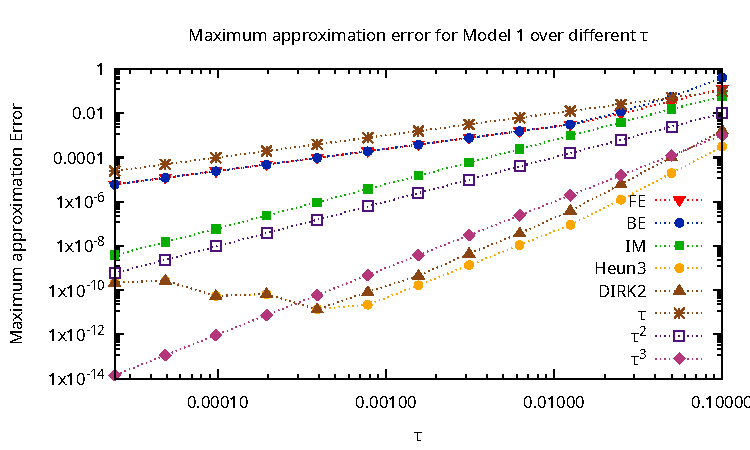
\includegraphics[width=1.0\textwidth]{ME_M1}
	\end{center}
	\caption{Graphical representation of the dependence of the maximum approximation error on the different time steps for model 1.
		\label{fig:Err_M1}}
\end{figure}

\begin{figure}[H]
	\begin{center}
		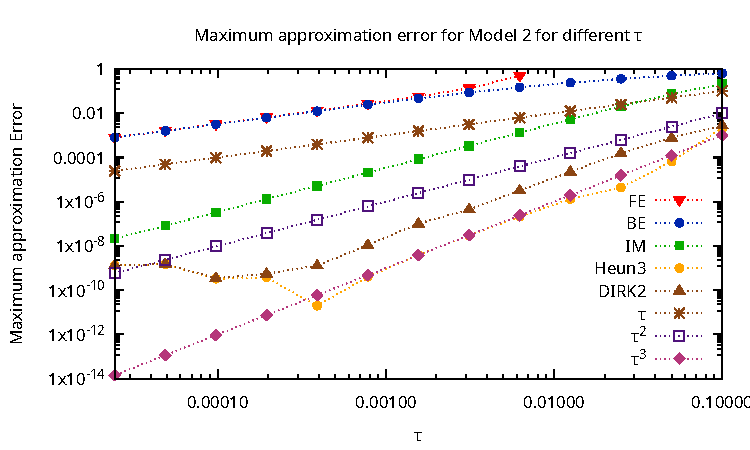
\includegraphics[width=1.0\textwidth]{ME_M2}
	\end{center}
	\caption{Graphical representation of the dependence of the maximum approximation error on the different time steps for model 2.
		\label{fig:Err_M2}}
\end{figure}

The plots confirm what has been previously stated through Thm.\ref{thm:zero-stability} and Thm.\ref{thm:order-cond-RK}. As a matter of fact, the good agreement between the $\tau$ and the profiles obtained for the FE and BE methods is clearly observable in Fig.\ref{fig:Err_M1} and Fig.\ref{fig:Err_M2}. It is also clear that the convergence error of the IM method is equal to 2. Moreover, the plots confirm what has been said above about the order of convergence of the DIRK2 method: its profile appears to be in good agreement with the theoretical profile $\tau^3$ and with the Heun3 one.\\

\subsubsection{Approximation error over time}
The approximation error, computed in the $L_\infty$ norm, has been studied as a function of the integration time for model 1 for two different step sizes, i.e. $h=0.1$ and $h=0.05$. The results are reported in the two following plots:

\begin{figure}[H]
	\begin{center}
		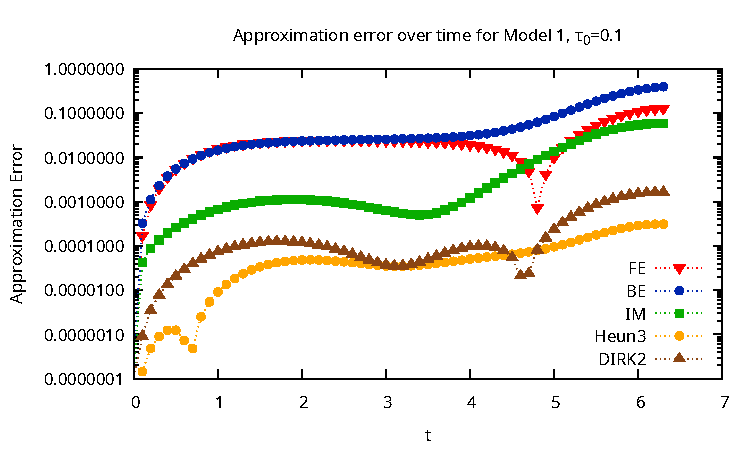
\includegraphics[width=0.85\textwidth]{Err_vs_t_1}
	\end{center}
	\caption{Graphical representation of the dependence of the approximation error on time for for model 1 and $h=0.1$.
		\label{fig:Err_vs_t_0_1}}
\end{figure}

\begin{figure}[H]
	\begin{center}
		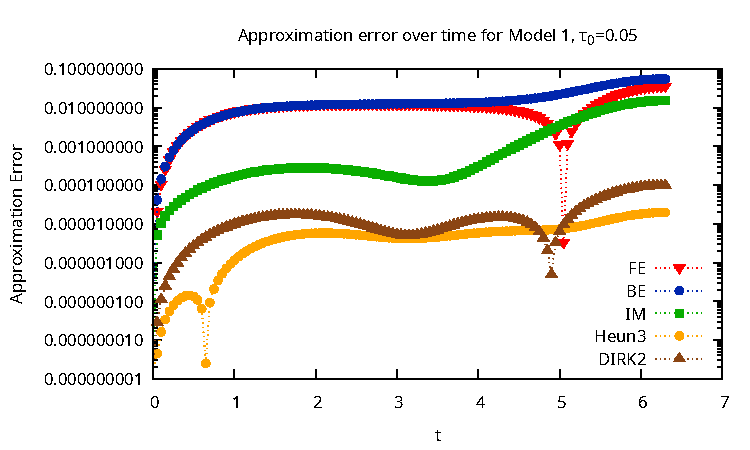
\includegraphics[width=0.85\textwidth]{Err_vs_t_05}
	\end{center}
	\caption{Graphical representation of the dependence of the approximation error on time for for model 2 and $h=0.05$.
		\label{fig:Err_vs_t_0_05}}
\end{figure}

Similar curves are observed in the plots. As expected, the error grows with time, even if, for specific and small time intervals, a decreasing profile is present.\\

\subsubsection{Efficiency of the methods}
A basic analysis of the performance of each of the methods is performed by means computing the number of times $f$ and $df$ are computed for each method. The results are output on the terminal so that a generic user can easily assess and verify them.\\
Unsurprisingly, the most performant method is represented by the FE method. This can be understood by noticing that method is an explicit one-stage method: usage of Newton's method is not required by the time evolution and the total number of evaluations of $f$ and $df$ is the minimum possible since no loops over $s$, $s$ being the number of stages of the method, is performed.\\

\section{Conclusive remarks}
In this section some additional comments and observation are presented.

\subsection{Memory}
As for the previous assignment, possible memory leaks have been checked.with the help of the software \emph{valgrind}, To do this, it is necessary to compile with \emph{-g} and \emph{-O1} optimisation. After having compiled the program, the following instruction has been used:


\begin{lstlisting}
$ valgrind --leak-check=yes ./adr
\end{lstlisting}


The following output has been produced on the terminal:

\begin{verbatim}
==31379== Memcheck, a memory error detector
==31379== Copyright (C) 2002-2017, and GNU GPL'd, by Julian Seward et al.
==31379== Using Valgrind-3.13.0 and LibVEX; rerun with -h for copyright info
==31379== Command: ./adr
==31379==
==31379== HEAP SUMMARY:
==31379==     in use at exit: 0 bytes in 0 blocks
==31379==   total heap usage: 244,730 allocs, 244,730 frees, 130,033,803 bytes allocated
==31379==
==31379== All heap blocks were freed -- no leaks are possible
==31379==
==31379== For counts of detected and suppressed errors, rerun with: -v
==31379== ERROR SUMMARY: 0 errors from 0 contexts (suppressed: 0 from 0)
\end{verbatim}

One can clearly see that no memory has been lost. This is however not surprising since no memory was dynamically allocated by the program and the correctness of the constructor for the SparseMatrix class was checked in the previous assignment.\\

\subsection{Performances}
\label{subsec:perf}
Performances can be checked through the following commands:
\begin{verbatim}
$ valgrind --tool=callgrind ./adr
$ kcachegrind
\end{verbatim}

The first command analyses the perfomances in the terms of load distrubution, while \emph{kcachegrind} is used to visualise the load distribution results. Differently from the previous case, performances depend on the code of the first assignment. The functions called within \emph{ADR$\_$Test} and \emph{Solver} are the ones taking up the majority of the time needed: unsurprisingly, \emph{Gauss-Seidel} is the most ``time-consuming" of them.\\


\cleardoublepage
%\add1contentsline{toc}{chapter}{\bibname}
\begin{thebibliography}{99}

\bibitem{numerical-math} A. Quateroni, R. Sacco, F. Saleri;
\emph{Numerical Mathematics}, Vol.37, Springer Verlag, (2007).

\bibitem{lec-notes} T. Grafke;
\emph{Scientific Computing}, Lecture Notes, University of Warwick, (2018).







\printindex
\end{thebibliography}
\bibliography{bibliography} % BibTeX database without .bib extension
\end{document}



%----------------------------------------------------------------------------------------
%	BIBLIOGRAPHY
%----------------------------------------------------------------------------------------

%\bibliographystyle{apalike}

%\bibliography{sample}

----------------------------------------------------------------------------------------


%end{document}